\documentclass[12pt]{report}
\usepackage[utf8]{inputenc}
\usepackage[russian]{babel}
%\usepackage[14pt]{extsizes}
\usepackage{listings}
\usepackage{graphicx}
\usepackage{amsmath,amsfonts,amssymb,amsthm,mathtools} 
\usepackage{pgfplots}
\usepackage{filecontents}
\usepackage{float}
\usepackage{indentfirst}
\usepackage{eucal}
\usepackage{enumitem}
\frenchspacing

\usepackage{indentfirst} % Красная строка


\usetikzlibrary{datavisualization}
\usetikzlibrary{datavisualization.formats.functions}

\usepackage{amsmath}




% Для листинга кода:
\lstset{ %
language=haskell,                 % выбор языка для подсветки (здесь это С)
basicstyle=\small\sffamily, % размер и начертание шрифта для подсветки кода
numbers=left,               % где поставить нумерацию строк (слева\справа)
numberstyle=\tiny,           % размер шрифта для номеров строк
stepnumber=1,                   % размер шага между двумя номерами строк
numbersep=5pt,                % как далеко отстоят номера строк от подсвечиваемого кода
showspaces=false,            % показывать или нет пробелы специальными отступами
showstringspaces=false,      % показывать или нет пробелы в строках
showtabs=false,             % показывать или нет табуляцию в строках
frame=single,              % рисовать рамку вокруг кода
tabsize=2,                 % размер табуляции по умолчанию равен 2 пробелам
captionpos=t,              % позиция заголовка вверху [t] или внизу [b] 
breaklines=true,           % автоматически переносить строки (да\нет)
breakatwhitespace=false, % переносить строки только если есть пробел
escapeinside={\#*}{*)}   % если нужно добавить комментарии в коде
}

\usepackage[left=2cm,right=2cm, top=2cm,bottom=2cm,bindingoffset=0cm]{geometry}
% Для измененных титулов глав:
\usepackage{titlesec, blindtext, color} % подключаем нужные пакеты
\definecolor{gray75}{gray}{0.75} % определяем цвет
\newcommand{\hsp}{\hspace{20pt}} % длина линии в 20pt
% titleformat определяет стиль
\titleformat{\chapter}[hang]{\Huge\bfseries}{\thechapter\hsp\textcolor{gray75}{|}\hsp}{0pt}{\Huge\bfseries}


% plot
\usepackage{pgfplots}
\usepackage{filecontents}
\usetikzlibrary{datavisualization}
\usetikzlibrary{datavisualization.formats.functions}

\begin{document}

\section*{Попытка спользования в md2 функции, определённой в md1}
При попытке использования локальной функции md1 в md2 возникает ошибка компиляции md2, так как в md2 нет ни объявления, ни определения функции (рис. \ref{03_res}).
\begin{lstlisting}[label=01_md1,caption=md1.c,language=C]
#include ...

static char *md1_proc_local(void)
{
	return md1_data;
}
...
\end{lstlisting}

\begin{lstlisting}[label=01_md2,caption=md2.c,language=C]
#include <..>
static int __init md_init(void) {
    
    printk("Module md2 was loaded\n");
    printk("Value returned from function md1_proc_local is : %s\n", md1_proc_local());
    return 0;
}
...
\end{lstlisting}

\begin{figure}[H]
	\centering
	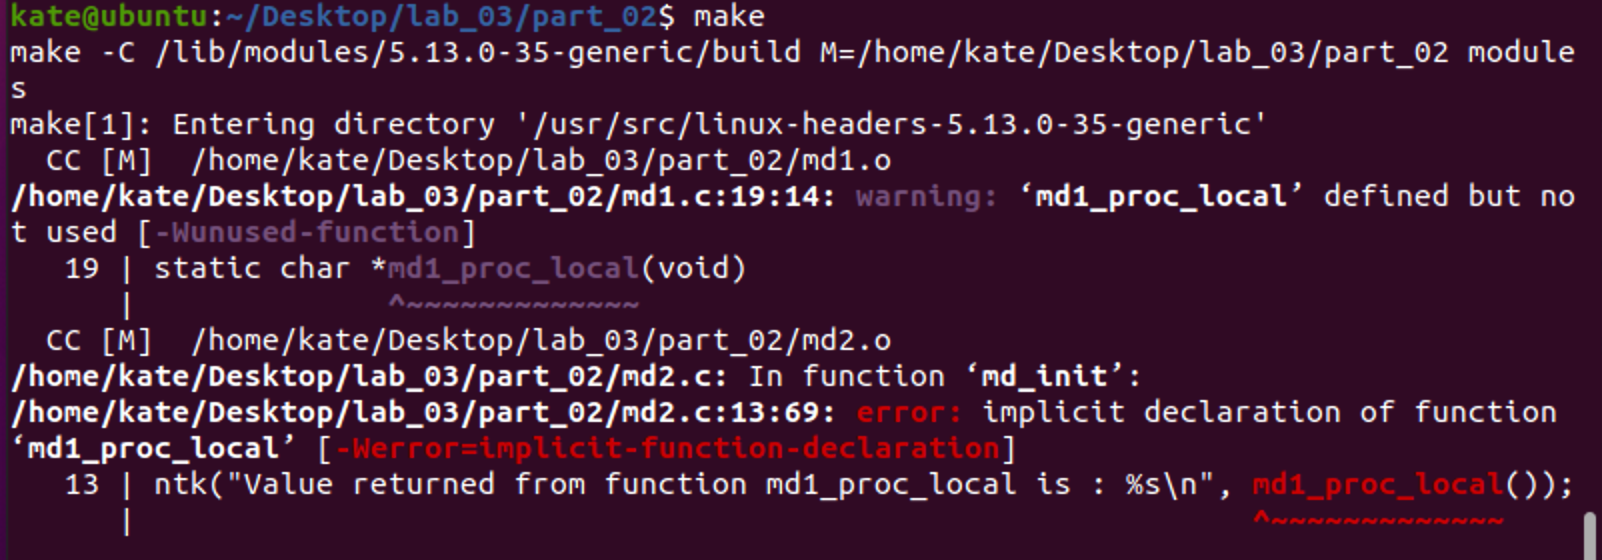
\includegraphics[scale = 0.6]{comp.png}
	\caption{Результат}
	\label{03_res}
\end{figure}
\newpage
\section*{Попытка экспортировать функцию из md1 в md2 без использования EXPORT\_SYMBOL}
Без EXPORT\_SYMBOL функция из md1 не была экспортирована в md2, так как на шаге MODPOST возникла ошибка отсутствия определения этой функции (рис. \ref{02_res}). 

Из документации про MODPOST:
\begin{figure}[H]
	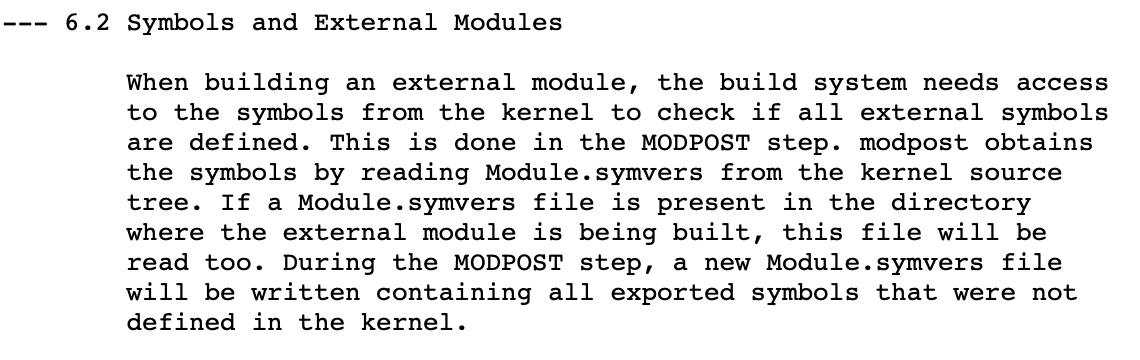
\includegraphics[scale = 0.8]{modpost.png}
	\caption{MODPOST step}
	\label{modpost_step}
\end{figure}

Таким образом, на шаге MODPOST проверяется, определены ли все внешние символы (система сборки обращается к символам из ядра). Так как макрос EXPORT\_SYMBOL не был применён к символу md1\_proc\_noexport, этот символ не попал в локальный Module.symvers файл, а значит не попал и в соответствующий файл ядра, поэтому проверка определения этого символа провалилась.

\begin{figure}[H]
	\centering
	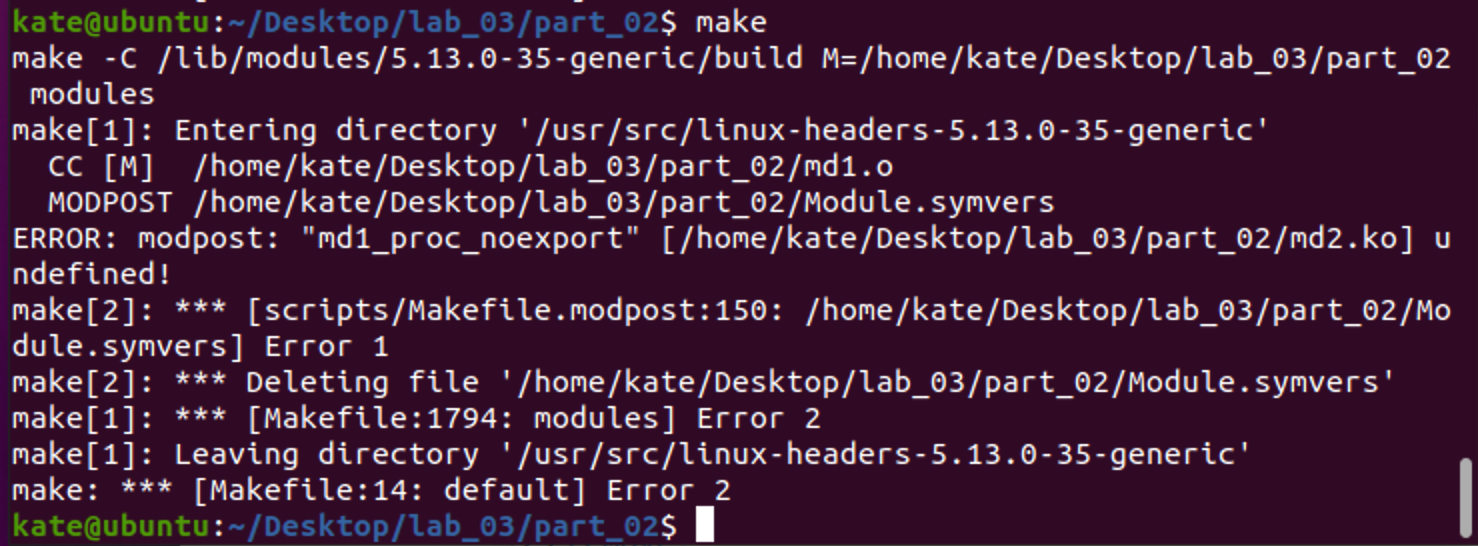
\includegraphics[scale = 0.6]{no_exp_symb.png}
	\caption{Результат}
	\label{02_res}
\end{figure}

\begin{lstlisting}[label=01_mdh,caption=md.h,language=C]
extern char *md1_proc_noexport(void);
\end{lstlisting}
\newpage
\begin{lstlisting}[label=01_md1,caption=md1.c,language=C]
#include "md.h"
#include ...

char *md1_proc_noexport(void)
{
	return md1_data;
}
...
\end{lstlisting}

\begin{lstlisting}[label=01_md2,caption=md2.c,language=C]
#include "md.h"
<..>
static int __init md_init(void) {
    
    printk("Module md2 was loaded\n");
    printk("Value returned from function md1_proc_noexport is : %s\n", md1_proc_noexport());
    return 0;
}
...
\end{lstlisting}
\newpage
\section*{Использование в md2 данных и функций, экспортированных с помощью EXPORT\_SYMBOL из md1}
При использовании EXPORT\_SYMBOL данные и функция были успешно экспортированы из md1 в md2, что подтверждается выводом в лог соответствующих сообщений (рис. \ref{01_res}).
\begin{lstlisting}[label=01_mdh,caption=md.h,language=C]
extern char *md1_data;
extern char *md1_proc(void);
\end{lstlisting}
\begin{lstlisting}[label=01_md1,caption=md1.c,language=C]
#include "md.h"
#include ...

char *md1_data = "md1_var_data";

char *md1_proc(void)
{
	return md1_data;
}
EXPORT_SYMBOL(md1_data);
EXPORT_SYMBOL(md1_proc);

...
\end{lstlisting}
\begin{lstlisting}[label=01_md2,caption=md2.c,language=C]
#include "md.h"
<..>
static int __init md_init(void) {
    
    printk("Module md2 was loaded\n");
    printk("Value exported from md1 : %s\n", md1_data);
    printk("Value returned from function md1_proc is : %s\n", md1_proc());
    return 0;
}
...
\end{lstlisting}

\begin{figure}[H]
	\centering
	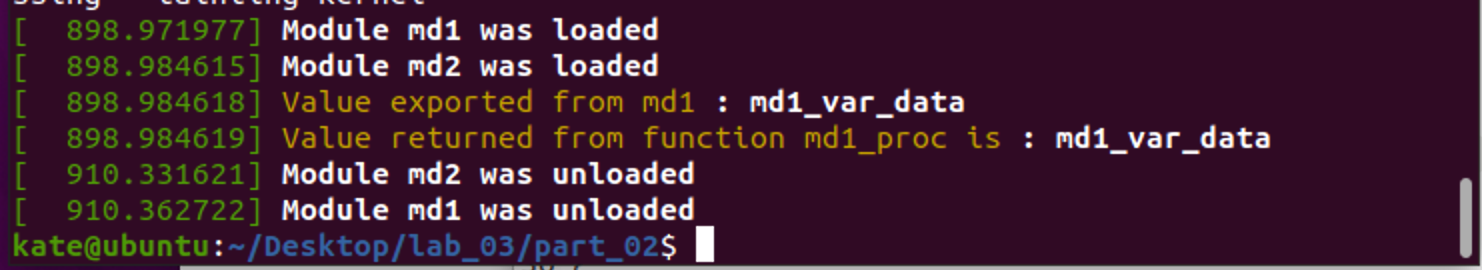
\includegraphics[scale = 0.6]{exp_symb.png}
	\caption{Результат}
	\label{01_res}
\end{figure}
\newpage
\section*{\_\_init возвращает -1}
В md3 используется код md2 из предыдущего пункта с изменением возвращаемого значения функции md\_init с 0 на -1, md1.c и md.h остались такими же. Сборка модулей прошла успешно, однако при загрузке возникла ошибка (рис. \ref{04_res}).

\begin{figure}[H]
	\centering
	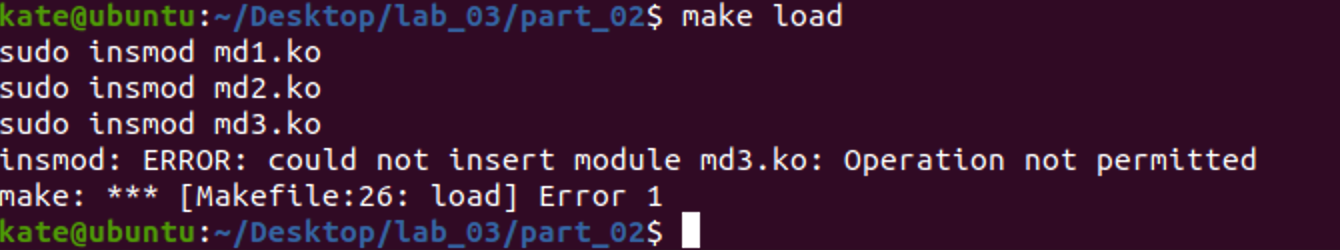
\includegraphics[scale = 0.6]{init_err.png}
	\caption{Результат}
	\label{01_res}
\end{figure}
\end{document}